
\documentclass[12pt,a4paper,pdftex]{article}

% packages
%%%%%%%%%%%%%%%%%%%%%%%%%%%%%%%%%%%%%%%%%%%%%%%%%%%%%%%%%%%%%
%%%%%%%%%%%%%%%%%%%%%%%%%%%%%%%%%%%%%%%%%%%%%%%%%%%%%%%%%%%%%

% Sprache
\usepackage[english]{babel}
\usepackage[utf8]{inputenc}

% Page layout
\usepackage{geometry}
\geometry{a4paper,lmargin={2.5cm}, rmargin={2.5cm}, tmargin={2.5cm}, bmargin={2.5cm}}

% figures
\usepackage{graphicx}
% Bilder importieren
\usepackage{epstopdf}
\epstopdfDeclareGraphicsRule{.pdf}{png}{.png}{convert #1 \OutputFile}
\DeclareGraphicsExtensions{.png,.pdf}
% Figure and Caption layout
\usepackage[bf]{caption}
\usepackage[list=true, font=large, labelfont=bf, 
labelformat=brace, position=top]{subcaption}\usepackage{wrapfig}
\usepackage{setspace}

% ABB. Verzeichnis (mehr Abstand zw. nummer und titel)
\usepackage{tocloft}
\setlength{\cftfignumwidth}{1.2cm}
\setlength{\cfttabnumwidth}{1.2cm}

% Befehle zur Textauszeichnung (hervorheben, unterstreichen ect.)
\usepackage{color,soul}
\usepackage{xcolor} % bunter Text

% Zitier-Style 
\usepackage{natbib}
\setcitestyle{author,year}
\usepackage[breaklinks=true,bookmarks=true,bookmarksopen=true,colorlinks=true,citecolor=gray,linkcolor=black,urlcolor=gray,pdfpagemode=UseNone,pdfstartview=FitH]{hyperref}

% other packages
\usepackage{float}
\usepackage{gensymb}
\usepackage{siunitx}
\usepackage{tabularx}
\usepackage{amsmath}
\usepackage{pgfgantt}
\usepackage{afterpage}
% für chemische zeichen
\usepackage[version=4]{mhchem}
\usepackage{upgreek}
% for commenting a whole section
\usepackage{verbatim}
% plus minus zeichen
\newcommand{\rpm}{\raisebox{.2ex}{$\scriptstyle\pm$} }


% Titelseite
%%%%%%%%%%%%%%%%%%%%%%%%%%%%%%%%%%%%%%%%%%%%%%%%%%%%%%%%%%%%%
%%%%%%%%%%%%%%%%%%%%%%%%%%%%%%%%%%%%%%%%%%%%%%%%%%%%%%%%%%%%%

\begin{document}
\setlength{\parindent}{0pt}

\begin{titlepage}
 \begin{center}
        \vspace{1cm}
        \Large
        Winter term 2019/2020\\
        Report of the master module: Großpraktikum
 
        \vspace*{4cm}
        \LARGE
        \textbf{Habitat Selection of Different Species of Gymnotiform Weakly Electric Fish}\\
        \vspace{0.25cm}
        \textbf{and}\\
        \vspace{0.25cm}
        \textbf{the Correlation with Dominance in \textit{A.~macrostomus} in LLanos of the Orinoco~Basin, Colombia}
        \vspace{5cm}
        
        \large
        Jacqueline Laura Göbl,\\ Julia Grüb,\\ Max Kühn
        \vspace{0.5cm}
        
        Supervisor: Prof. Dr. Jan Benda
        
        \vfill
        \large     
        T\"ubingen, \today
    \end{center}
    
    %\newpage
    %    \thispagestyle{empty}
    %    \mbox{}
    %    \newpage
\end{titlepage}


\thispagestyle{empty}
\mbox{}


% Inhaltsverzeichnis
%%%%%%%%%%%%%%%%%%%%%%%%%%%%%%%%%%%%%%%%%%%%%%%%%%%%%%%%%%%%%%
%%%%%%%%%%%%%%%%%%%%%%%%%%%%%%%%%%%%%%%%%%%%%%%%%%%%%%%%%%%%%%

\tableofcontents
\thispagestyle{empty}

% Textbegin
%%%%%%%%%%%%%%%%%%%%%%%%%%%%%%%%%%%%%%%%%%%%%%%%%%%%%%%%%%
%%%%%%%%%%%%%%%%%%%%%%%%%%%%%%%%%%%%%%%%%%%%%%%%%%%%%%%%%
\newpage
\section{Introduction}
There  are  arguably  few  places  in  the  world  that  can  claim  a biodiversity as high as Colombia’s. Colombia’s unique ecosystem is comprised of numerous animal species that have adapted to a diverse set of habitats. Among these, weakly electric fish make up \~80\%  of the biomass of the respective native fish fauna \citep{marrero1991notas}. The south American weakly electric fish belong to the order of Gymnotiformes, with five known families and 135 different species (current state \citeyear{albert2005diversity}, \citeauthor{albert2005diversity}).

The weakly electric fish evolved an electric organ which cells discharge simultaneously and create an electric field around the animal \citep{Zupanc_Bullock_2005}. They use this electric organ discharge (EOD) for electrolocation, orientation and object recognition \citep{Heiligenberg_73}, communication \citep{Hopkins_74} and foraging \citep{Nelson_MacIver_1999}. Amongst the weakly electric fish two types of EOD are known. Wave-type fish emit a continuous, quasi sinusoidal EOD with a constant frequency, while pulse-type fish emit very brief stereotyped pulses, with varying inter-pulse-intervals \citep{Zupanc_Bullock_2005}.
The electric organ discharge is 
not only different between these two types, it also differs between species, i.e. in their waveforms and their EOD frequencies \citep{Zupanc_Bullock_2005}.
% about ecletric organ and how it represents the dominance in males (A.apteronotus)
Also differences in EOD frequency between individuals of the same species can be found. This differences in frequency are known as indicating dominance among males \citep{HAGEDORN1985}.\\

\begin{figure}
    \centering
    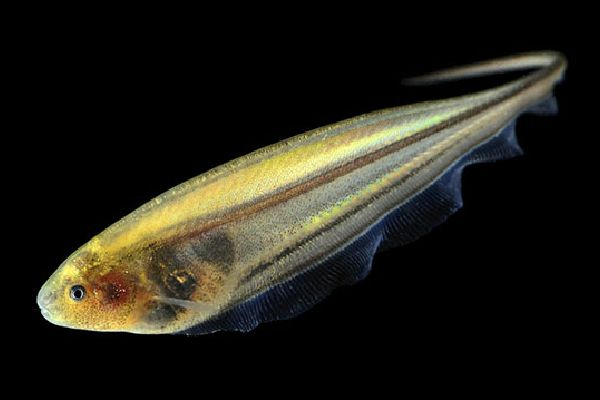
\includegraphics[width = \textwidth]{pictures/Eigenmannia_virescens.jpg}
    \caption{\textit{\textbf{Eigenmannia virescens.}} Picture of a cute weakly electric fish of the species \textit{Eigenmannia virescens} from a questionable, Russian website: \url{http://aquavitro.org/2014/11/13/vidy-ryb-nozhej/} (30.01.2020).}
    \label{fig:eigenmannia_cute}
\end{figure}

Previous studies have shown that dominance strongly influences the inhabitation of shelters \citep{raab2019}.
Which is relevant for the animal's survival, since weakly electric fish hide during the day \citep{Hopkins_74}.     
In staged laboratory settings it could be shown that dominant males, with the highest EOD frequencies, defend the best shelters against subordinate males \citep{raab2019}.
It could also been shown that, at least for some species, male individuals are more likely to defend their shelters against same sex conspecifics. In contrast, females are more likely to share shelters with their conspecifics \citep{dunlap2002retreat}.
A relation between shelter, or more general habitat selection, was also already shown for other species within the animal kingdom, i.e. aquatic species like salmons \citep{redsalmon1995}, but also in terrestrial species, like redstarts \citep{sherry1989redstarts} or lizards \citep{downes1998heat}.
In general it is known, that different species prefer different habitats. However, for each species the preferred or most attractive habitat can depend on other characteristics.
In case of weakly electric fish, some species prefer to seek shelter between roots (\textit{Eigenmannia}, \citeauthor{Hopkins_74}, \citeyear{Hopkins_74}), under sunken rocks Gymnotus, \citeauthor{westby1988ecology}, \citeyear{westby1988ecology}), in leaf litter (Brachyhypopomus, \citeauthor{hagedorn1988ecology}, \citeyear{hagedorn1988ecology}) or even in sand (Gymnorhamphichthys, \citeauthor{lissmann1965activity}, \citeyear{lissmann1965activity}).
For aquatic species, the most attractive habitat can also depend on water flow or water depth \citep{aadland1993stream}.
% was wir getan haben und warum
While gymnotiform weakly electric fish are well researched in the lab and their dominance behaviour as well, much less is known about the ecology and ethology of these animals in the wild. 
Therefore, first conditions of their natural habitat in the LLanos of the Orinoco basin, in the Reserva el Caduceo in San Martin, Meta, Colombia were characterised. 
Second, the occurring species of Gymnotiformes, \textit{Apteronotus macrostomus, Eigenmannia virescens} and gymnotiform pulsefish, and their density in these habitats were sampled.
Between the species, their occurrence densities, dependent on the habitat characteristics, were compared in order to detect possible habitat preferences.
Additionally, for the species \textit{A. macrostomus} the EOD frequency, which is correlated with dominance, was compared within the inhabited habitats. Since, dominance between territorial males might not only determine their fitness but might also influence selection of resting sites, because better resting sites might reduce physiological costs.
Summarised, our research questions were:\\

\begin{itemize}
\item[1.] What are the environmental conditions (ground conditions, water flow and depth) of the natural habitat of gymnotiform weakly electric fish?

\item[2.] Do different species of weakly electric fish prefer different habitats conditions?

\item[3.] Does the social dominance influences the  habitat selection in \textit{A. macrostomus}?
\end{itemize}{}
 

\newpage
\section{Methods}
\subsection{Recordings}
\label{sec:recordings}

\textit{Recording site}: To gain information about the habitats of different species of weakly electric fish, we did field recordings in in a tropical grassland plain in the Rio Canocamoa, which is located in the LLanos of the Orinoco basin in the Reserva el Caduceo, San Martín, Departement del Meta in Colombia (fig.~\ref{fig:map}). This area is composed of branched networks of smaller streams and larger rivers.
The measured habitats were chosen dependent on their individual characteristics to gain as much habitat diversity as possible. Thus the habitats varied in water depth, water flow and structure of the ground and the shoreline. During the recording period in early October, right after the rain season, the average water temperature was 25.6 \rpm \ang{1.02}C. The average water conductivity was 9.78 \rpm 4.48 $\frac{\mu S}{cm}$.

\begin{figure}[H]
    \centering
    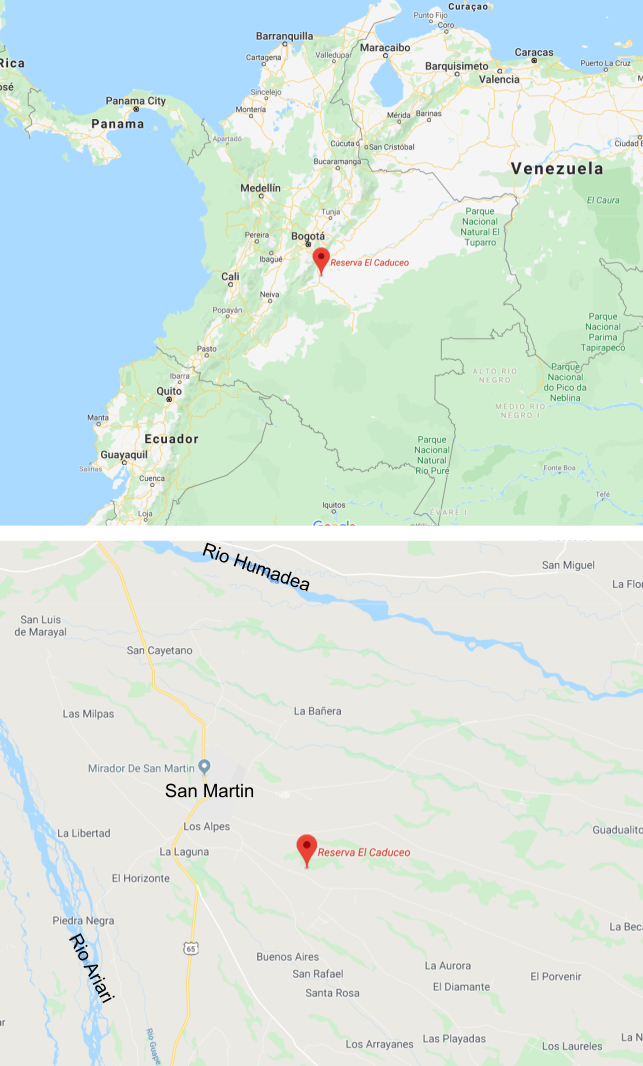
\includegraphics[width=0.58\textwidth]{pictures/Methods/map.png}
    \caption{\textbf{Location Reserva el Caduceo, Colombia.} \textbf{Top:} Location of the Reserva el Caduceo (red) within Colombia. \textbf{Bottom:} Location of the reservation within the Orinoco basin. \url{(https://goo.gl/maps/J3h9ntWjrADx44Sx6, 29.01.2020)}}
    \label{fig:map}
\end{figure}{}

\textit{Recording procedure}: In order to record the electric fields of the fish, self-made fishfinder were used. These consisted of a PVC-rod with an lead electrode on the top and a reference electrode on the bottom (fig.~\ref{fig:fishfinder}). The recorded signal was amplified with an audio amplifier of the brand RadioShack, and recorded via a MP3 player (Trancend’s MP330).
In case of many fish all-around the habitat, the recordings were made systematically, every 1-2 m (fig.~\ref{fig:habitats}~BE). Regular distances were chosen to avoid resampling of individual fish and to cover larger areas. Also, the fishfinder was positioned close to one fish within these recording areas. In case of only a few fish within the habitat, the recordings were made at the positions of each fish (fig.~\ref{fig:habitats}~ACD). Each individual recording within a habitat refers to a micro-habitat. For each measurement’s position the micro-habitat’s characteristics, such as the presence or absence of sand, mud, plants, roots and stones, were documented. The stones were further characterised as stacked or not stacked. Furthermore the water depth and the water flow (Advanced Stream Flowmeter by GEOPACKS) was measured. These characteristics were noted for micro-habitats in which fish were found, as well es for for areas without any detectable fish.
Over all, within 13 different habitats, 19 micro-habitats without detectable weakly electric fish and 139 different micro-habitats with weakly electric fish were found, characterised and recorded.

\begin{figure}[H]
    \centering
    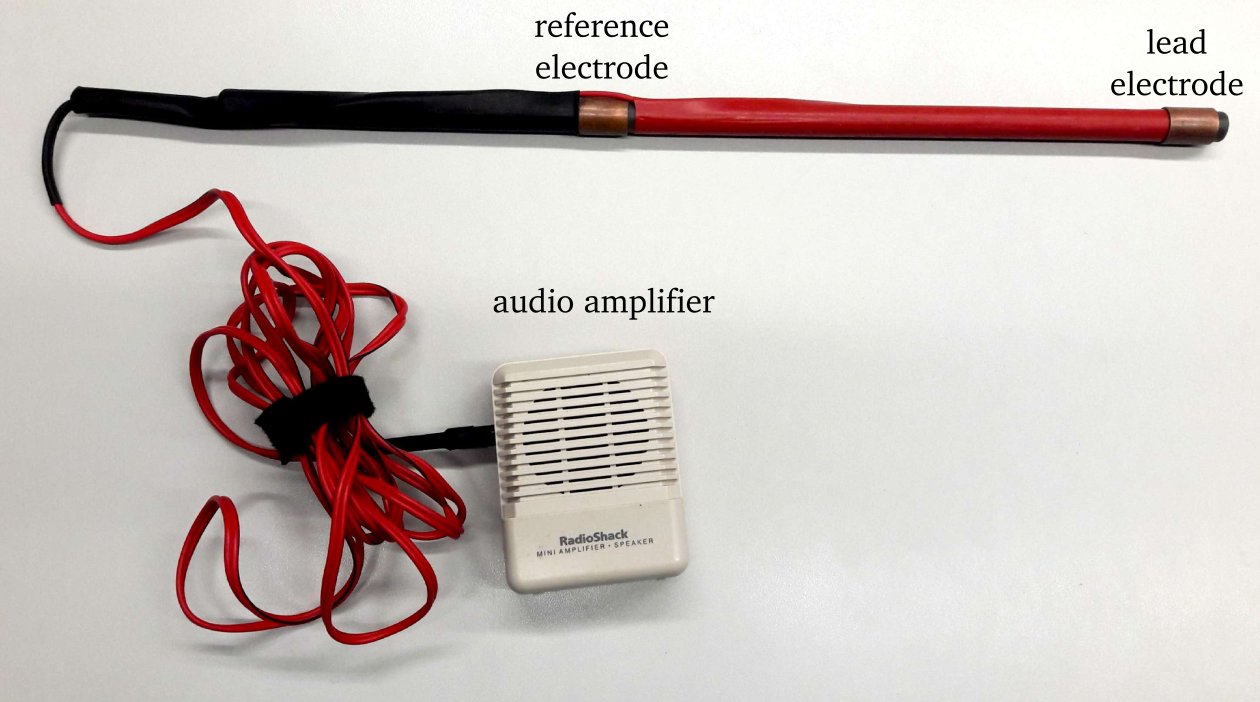
\includegraphics[width=\textwidth]{pictures/Methods/fishfinder.png}
    \caption{\textbf{Self-made fishfinder and audio amplifier of the brand RadioShack}}
    \label{fig:fishfinder}
\end{figure}{}

\begin{figure}[H]
    \centering
    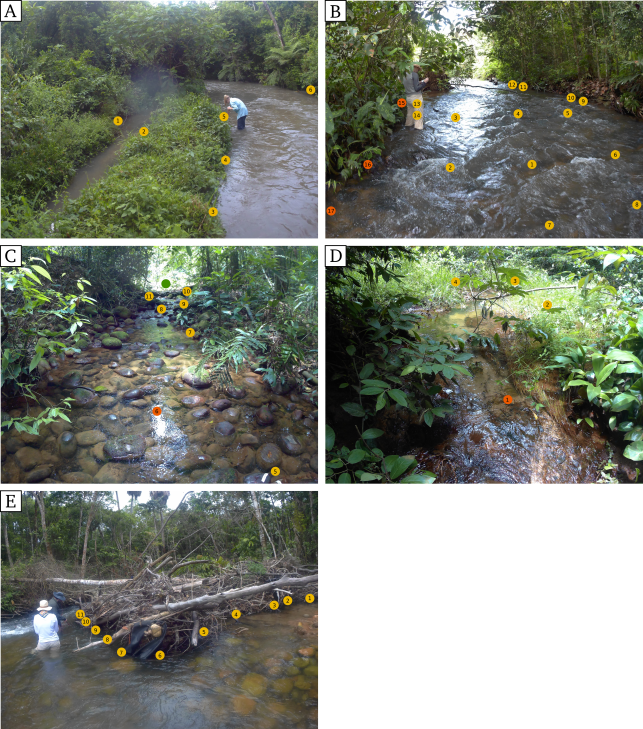
\includegraphics[width = 0.9\textwidth]{pictures/Methods/all_habitats.png}
    \caption{\textbf{Five example recording habitats in the reservoir El Caduceo, with each recording site (micro-habitat). A:} On the left: small muddy side stream with two micro-habitats (yellow dots: 1 \& 2), on the right: large fast river with four recording sides (3~-~6). \textbf{B:} The same river as in A further downstream, with fourteen micro-habitats with fish (yellow) and three micro-habitats without fish (orange, 15~-~17). \textbf{C:} A clear, stony side stream with six micro-habitats with fish (yellow) and one 'no fish area' (orange, 6). The adjacent habitat D is marked with a green dot. \textbf{D:} Further up in the side stream of habitat C, this habitat is composed of a muddy underground with many plants. In hree of the micro-habitats fish were found (yellow, 2~–~4), in one micro-habitat no fish were found (orange, 1). \textbf{E:} Eleven recording sites systematically along a wooden dam in a large river.}
    \label{fig:habitats}
\end{figure}

\subsection{Sorting Species}
In order to analyse the (micro-)habitat preference of different species of weakly electric fish, the first task was to determine how many fish were actually in each of  the recordings. Therefore, with the program thunderfish ($\copyright$ Benda-Lab) each recording was analysed and based on the power spectrum, the EOD and waveform for each individual fish was calculated.
Dependent on the EOD waveform the fish were categorised into wave- and pulse-type fish. Pulse-type fish weren't further separated into different species. To further separate the wave-type fish into different species, different EOD parameters were extracted with the program collectfish ($\copyright$ Benda-Lab). On the basis of the EOD frequency and the relative peak amplitude (RPA), the fish's EOD were separated into three clusters, each corresponding to one endemic species: \textit{Apteronotus macrostomus} \citep{Santana2013}, \textit{Sternopygus macrurus} \citep{Keller1991} and \textit{Eigenmannia virescens}~\citep{silva2009cytogenetic}. According to the literature the EODf of Sternopygus ranges from 50~-~200~Hz \citep{Keller1991}, the EODf of \textit{Eigenmannia} from 250~-~600~Hz \citep{Hopkins_74}, while the EODf of adult Apteronoti ranges from 600~-~1000~Hz. The EODf of juvenile Apteronoti ranges from 400 to 600~Hz \citep{Meyer1987}.
Within the critical EODf window of 250~-~577~Hz, where the EOD frequencies of \textit{Apteronotus} and \textit{Eigenmannia} overlap, the fish species couldn't be determined easily. Since both species differ in their EOD waveform, waveform characteristics were used to discriminate between these two species within the critical range: The waveform of \textit{Eigenmannia} and \textit{Apteronotus} differ in the aspect of the relative peak amplitude (RPA). The RPA of \textit{Apteronotus} is more or less 1, since the EOD is a biphasic signal \citep{Zupanc_Bullock_2005} (fig.~\ref{fig:EOD_waveforms}). The waveform of \textit{Eigenmannia}, however, is monophasic \citep{Zupanc_Bullock_2005} with a slightly shifted zero line towards the negative. Therefor, the amplitude of the minimum is about the half of the amplitude of the maximum. Consequently, the RPA of \textit{Eigenmannia} is 0.5 (fig.~\ref{fig:EOD_waveforms}). Based on the distribution of the clusters and the waveform characteristics, the boundary was placed at a relative peak amplitude of 0.72 (fig.~\ref{fig:cluster}). However, regarding the waveforms of the individual Apteronoti with EOD frequencies below 500~Hz, the waveforms did not show the typal characteristics. Accordingly, these individuals were excluded from further analysis. Since only two individuals of the genus Sternopygus were recorded, these individuals were also excluded from the analysis.

%%\item  \textcolor{gray}{how many fish of a given species were present in each of the \textcolor{red}{???} recordings. Therefor, for each individual fish of each recording the EOD characteristics were analyzed with/by the program thunderfish ($\copyright$ Benda-Lab).   Within an analyzing window of 8s this program calculates the average EOD waveform (n=1000) and its power spectrum for each individual fish. Individuals with a power less then -60 dB were not analyzed.   Waveforms of fish, that were orientated tail first to the recording electrodes, were flipped in amplitude. For the pulse-fish only the EOD frequency (EODf) was analyzed.  For the wave-fish EOD parameters, such as fundamental or EOD frequency, frequency of the harmonics and their amplitudes and phases, were calculated. Other EOD characteristics, i.e. peak to peak amplitude, relative peak amplitudes and peak to peak distance  then: plot this characteristics against each other to search for clusters to determine species habitat characteristica + species for each individual fish in the recordings wave-type fish  Apteronotus leptorhynchus EODf: 600-1100 Hz (Meyer, 1973 and \cite{Hopkins_74}) ! juveniles lower in EODf: can be down to 400-500 Hz (Meyer, 1973) Eigenmannia EODf: 240-600 Hz (Meyer, 1973 and \cite{Hopkins_74}) Sternopygus EODf: 50-150 Hz (Meyer, 1973 and \cite{Hopkins_74}) Critical Freqency = 400 – 600 Hz (Eigenmannia vs. Apteronotus) to determine which waveform belongs to which species, different waveform characteristics were plotted against each other  Parameter 1 (EODf): Sterno < 250 Hz < Eigenmannia < 577 Hz < Apteronotus Parameter 2 (relative peak amplitude): amplitude of minimum relative to amplitude of maximum 72 \% Within the critical EODf window of 250~-~577~Hz the fish species couldn't be determined easily. The waveform of Eigenmannia and Apteronotus differ in the aspect of the relative peak amplitude, regarding that the relative peak amplitude of Apteronotus is more or less 1 since it is a biphasic (\textcolor{red}{Quelle}) signal around 0 (\textcolor{red}{Quelle}). The waveform of Eigenmannia however, is monophasic (\textcolor{red}{Quelle}) with a slightly shifted zero line towards the negativ (\textcolor{red}{Quelle}). Therefore the amplitude of the minima is about the half of the amplitude of the maxima.}

\begin{figure}[H]
    \centering
    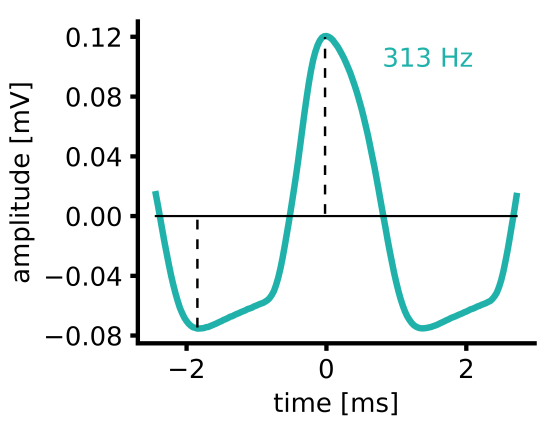
\includegraphics[width=0.496\textwidth]{pictures/Methods/waveform_eig.png}
    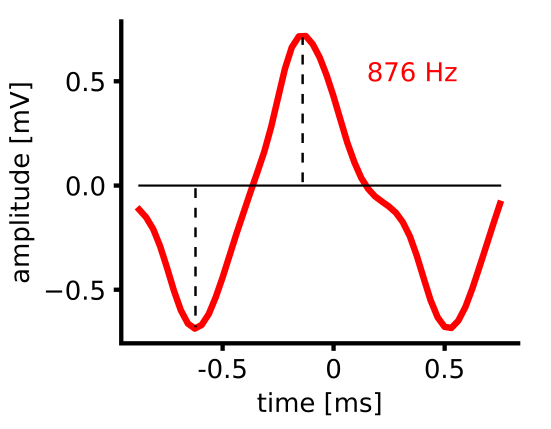
\includegraphics[width=0.496\textwidth]{pictures/Methods/waveform_apt.png}
    \caption{\textbf{EOD waveform of \textit{Apteronotus} and \textit{Eigenmannia}.} Shown are exemplary EOD waveforms of individuals of the species \textit{Eigenmannia} (cyan), with an EOD frequency of 313~Hz, and \textit{Apteronotus} (red), with an EODf of 876~Hz. The amplitudes of the positive and negative peaks are marked with dashed lines.}
    \label{fig:EOD_waveforms}
\end{figure}{}

\begin{figure}[H]
    \centering
    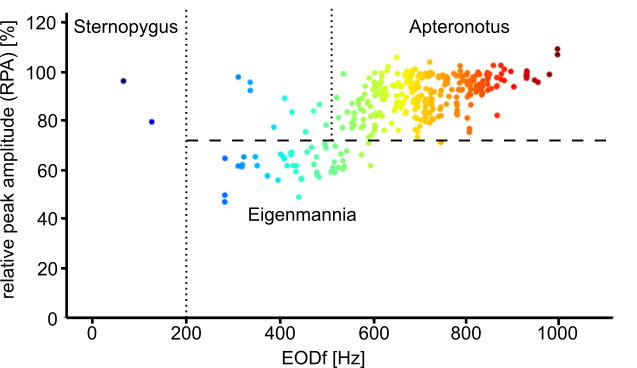
\includegraphics[width=0.9\textwidth]{pictures/Methods/cluster.png}
    \caption{\textbf{Determination of wave-type species dependent on RPA and EODf.} Shown is the relative peak amplitude (RPA) and the EOD frequency of each recorded animal. The color corresponds to the EODf. Fish with a EODf lower than 200~Hz were identified as Sternopygus. The differentiation between \textit{Apteronotus} and \textit{Eigenmannia} was based on the RPA. Animals with a RPA lower than 0.72 were classified as \textit{Eigenmannia}. Animals with a RPA greater than 0.72 as \textit{Apteronotus}. Since, the waveform of the Apteronoti with an EODf lower than 500~Hz was typal, these individuals were excluded from further analysis.}
    \label{fig:cluster}
\end{figure}{} 


\newpage
\section{Results}
% ------------------------------------------
% habitat count  & fish count 
% ------------------------------------------

\subsection{Habitat characteristics and preferences}

To answer the question if different species or genera of weakly electric fish prefer different habitat characteristics, weakly electric fish were recorded in a network of river channels in the LLanos of the Orinoco basin, Meta, Colombia. For each recording the microhabitat's characteristics were categorised. In total, within 13 larger habitats, 139 microhabitat's characteristics, such as the presence or absence of stones, sand, mud, roots and plants, were denoted.\\
Within most (115~microhabitats, 83~\%) of the examined microhabitats stones were frequently found on the ground (fig.~\ref{fig:habitat_count}). In 47 microhabitats  (34~\%) the stream bed was additionally or solely covered with sand. Roots were often (62~microhabitats,~45~\%) found on the shoreline, on the ground or as locked driftwood. Both, mud (7~microhabitats,~5~\%) and plants (14~microhabitats,~10~\%), were clearly less frequent than other examined characteristics.\\
For each microhabitat the species or genus of each recorded fish was determined. Over all, 327 weakly electric fish were recorded. \textit{Apteronotus} was by far the most frequent species. Approximately 250 of the recorded animals (76~\%) were identified as \textit{Apteronotus macrostomus} (fig.~\ref{fig:fish_count_eod}~A). The EOD frequency of these animals ranged from approximately 560~to 1000~Hz and was slightly trimodal distributed (fig.~\ref{fig:fish_count_eod}~B). About 50 fish (15~\%) were identified as \textit{Eigenmannia virescens}. Their EODf mainly varied from 290~to 600~Hz. With 20~(6~\%) recorded individuals pulsefish were by far the least frequent. The EODf of this genus is less than 100~Hz.

\begin{figure}[H]
    \centering
    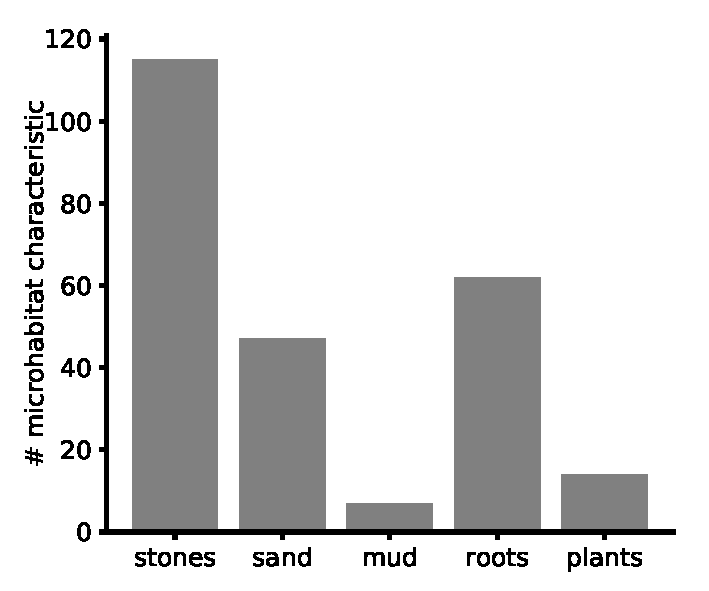
\includegraphics[width=0.7\textwidth]{pictures/Results/JULE_habitat_ccharacteristics.pdf}
    \caption{\textbf{Habitat characteristics.} Total count of the different microhabitat characteristics: stones, sand, mud, roots or different kinds of plants. A single microhabitat could consist of multiple of these categories. Over-all, 139 microhabitats were characterised.}
    \label{fig:habitat_count}
\end{figure}

\begin{figure}[H]
    \centering
    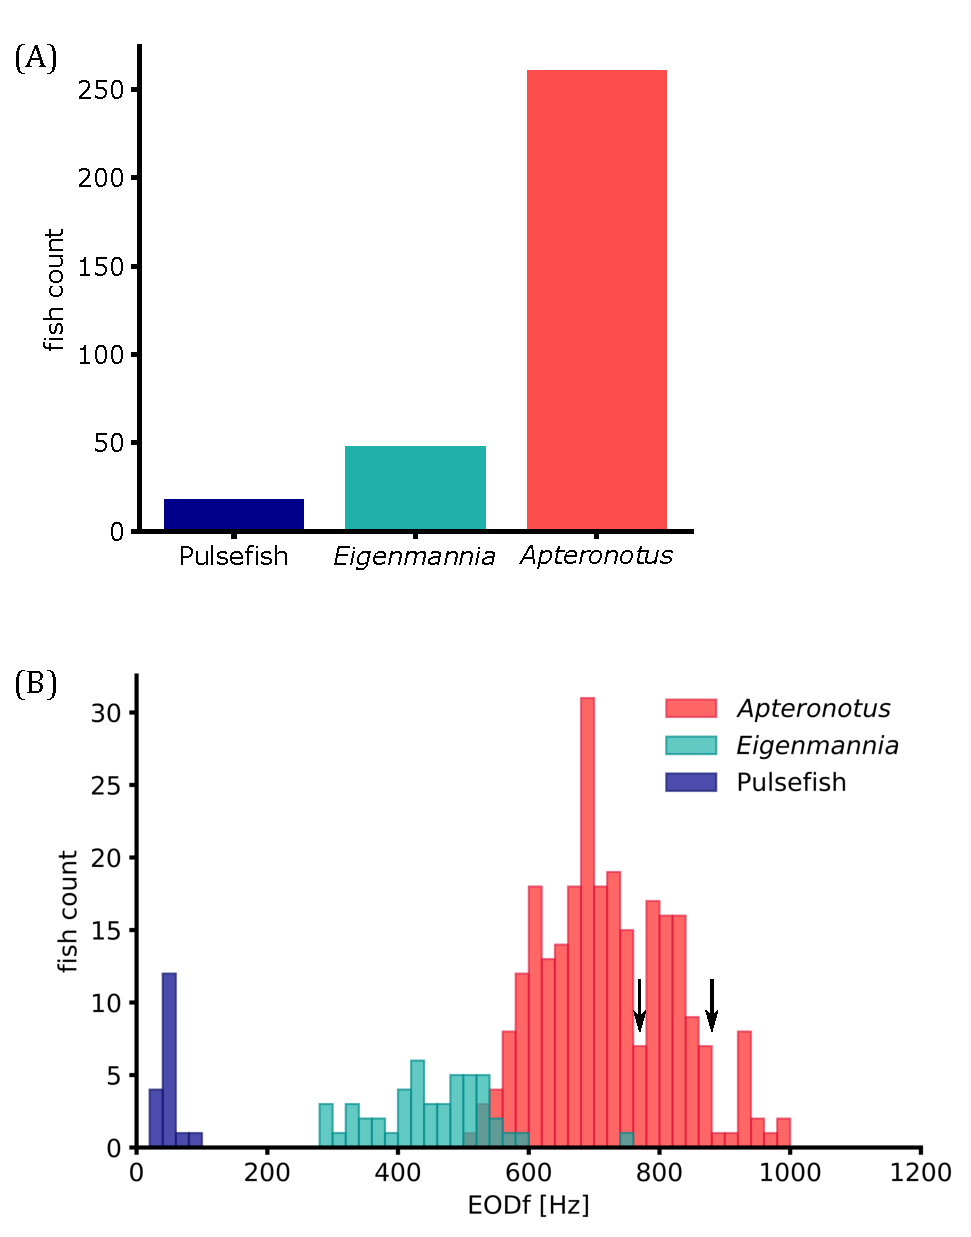
\includegraphics[width=0.9\textwidth]{pictures/Results/fish_count_EOD.pdf}
    \caption{\textbf{Proportion of fish species and EOD distribution.} \textbf{A:}~Shown is the number of animals that were recorded within the 139 investigated microhabitats for each species (\textit{Apteronotus macrostomus} and \textit{Eigenmannia virescens}) or genus (pulsefish). \textbf{B:}~Distribution of the EOD frequencies (EODf) for each species or genus. In case of \textit{Apteronotus}, the first arrow (762~Hz) indicates the border between female and male individuals. The second arrow (880~Hz) marks the border between males with lower EODf (lower dominance) and higher EODf (highly dominant males).}
    \label{fig:fish_count_eod}
\end{figure}

% ---------------------------------------------
% species and habitats
% ---------------------------------------------

Regarding the average fish count dependent on the microhabitat characteristics, some differences between the different species or genera can be seen, especially regarding \textit{Apteronotus} (fig.~\ref{fig:habitat_count_species}). On average, in each microhabitat containing stones, two \textit{Apteronoti} were found. Close to roots on average only one \textit{Apteronotus} was found. In microhabitats with sand, mud and plants, this species was less frequent.
Most \textit{Eigenmannia}s were found in habitats with roots. On average the probability of finding an \textit{Eigenmannia} within a microhabitat with roots was 75~\%. The probability of finding an individual of this species within a stony, sandy or muddy habitat reached from 25~to 50~\%. Not a single animal was found in a microhabitat containing plants.
In contrast, most of the pulsefish, with a probability of 70~\%, were found in habitats with plants. The probability of finding a pulse-type fish within a microhabitat containing sand, mud or roots ranged between 25~and 50~\%. Pulsefish were the less frequent in stony habitats.

\begin{figure}[H]
    \centering
    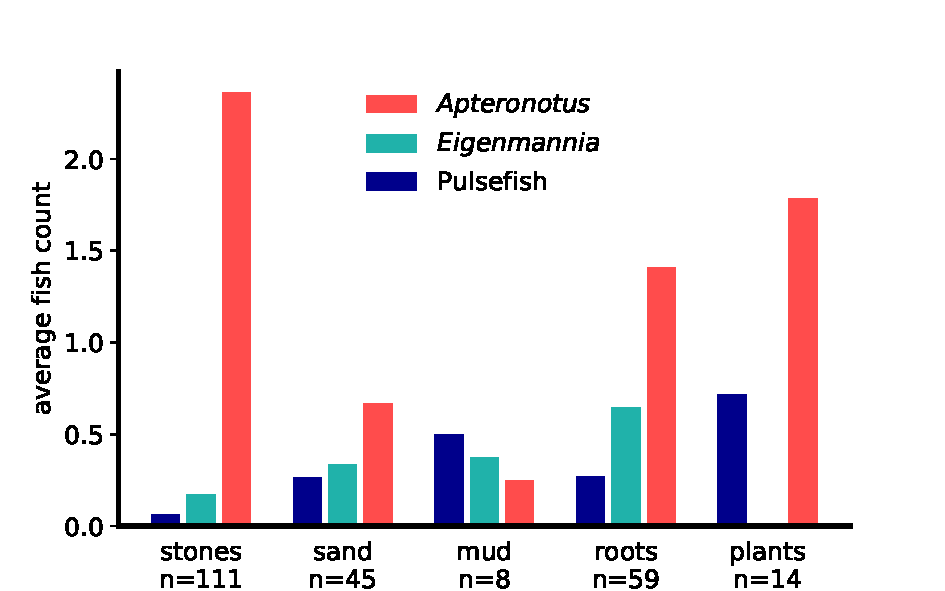
\includegraphics[width = \textwidth]{pictures/Results/average_occuranec_in_habitats.pdf}
    \caption{\textbf{Occurrence of species in the different microhabitats.}
    Shown is the average fish count of Pulsefish (blue), \textit{Eigenmannia virescens} (cyan) and \textit{Apteronotus macrostomus} (red) in an microhabitat with certain characteristics. Microhabitats could contain many different characteristic elements. Hence, a single microhabitat and the corresponding recorded animals can occur more than once in the figure. The average fish count corresponds with the occurrence probability in a microhabitat with a certain characteristic.}
    \label{fig:habitat_count_species}
\end{figure}

\begin{figure}[H]
    \centering
    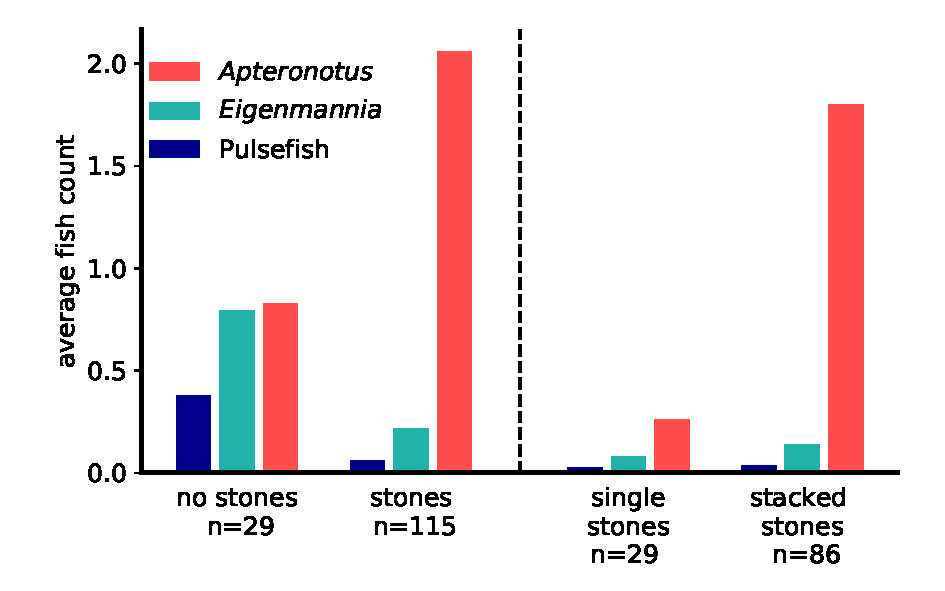
\includegraphics[width = \textwidth]{pictures/Results/more_stones_pls.pdf}
    \caption{\textbf{Occurrence of species in stony habitats.} Shown is the average fish count for Pulsefish (blue), \textit{Eigenmannia virescens} (cyan) and \textit{Apteronotus macrostomus} (red) for microhabitats with and without stones (left). Stony microhabitats are further subdivided into single stones or stacked stones (right). The average fish count corresponds with the occurrence probability in a microhabitat with a certain characteristic.}
    \label{fig:habitat_count_stones}
\end{figure}

Next, we solely looked at the occurrence of the fishes in stony habitats and in habitats without stones (fig.~\ref{fig:habitat_count_stones}). \textit{Eigenmannia} and pulsefish occurred more often in microhabitats without any stones. The probability of finding an individual of the species \textit{Eigenmannia} in a stony microhabitat was 22~\%, for pulsefish 5~\%. Regarding stony habitats, both occurred with the same frequency, regardless whether there were single or stacked stones. Both occurred with a probability of less than 13~\%. In contrast, \textit{A. macrostomus} was clearly more frequent in stony habitats. On average in each stony habitat two individuals of this species were found. In habitats without stones on average only less than one individual was found. A comparison between habitats with single and stacked stones shows, that \textit{Apteronotus} was by far most often found in microhabitats containing stacked stones, with an average fish count of 1,7~individuals per microhabitat.

\begin{figure}[H]
    \centering
    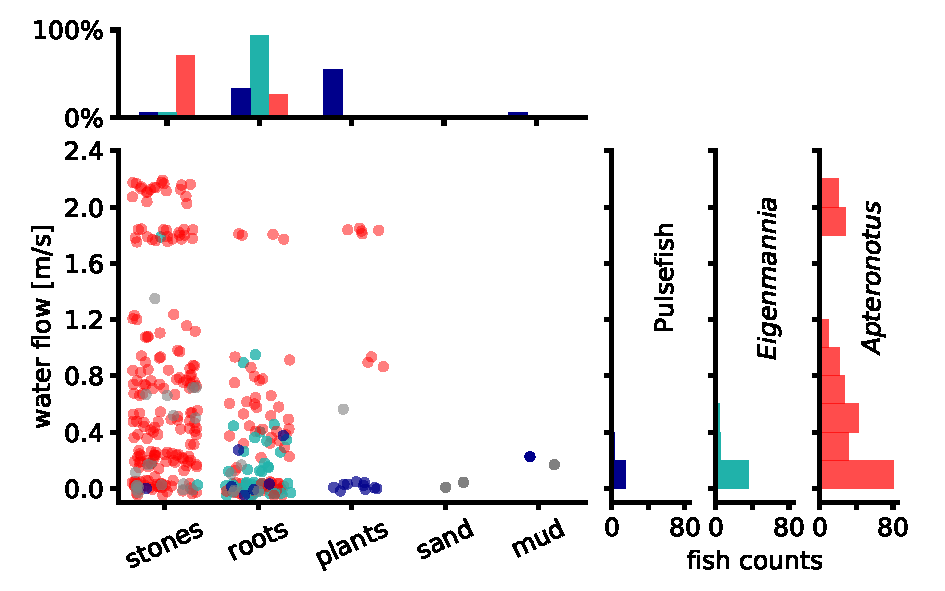
\includegraphics{pictures/Results/flow_habitat_protocol.pdf}
    \caption{\textbf{Distribution of the different fish species over the water flow in different microhabitats.} On the top, for the species \textit{Apteronotus} (red) and \textit{Eigenmannia} (cyan) and the genus of pulsefish (blue) the distribution in the different habitats is shown. The bottom left figure shows the distribution of the fishes in the different habitats over the water flow. The areas with no recorded fish (grey) are shown as well. The habitats are ranked according to the observations in the field. Habitats with roots were ranked above stones, while plants are ranked above roots. If there were neither roots nor plant nor stones, mud was preferred over sand (plants~$>$~roots~$>$~stones~$>$~mud~$>$~sand). The three histograms on the bottom right, show the distribution of the species over the water flow.}
    \label{fig:habitat_vs_flow}
\end{figure}

In contrary to the previous results, in figure~\ref{fig:habitat_vs_flow} every fish is only represented once. Additionally, different microhabitats are ranked based on the observation of the experimenter. The ranking considered that plants are preferred over roots, but if there are no roots and plants, stones were preferred over mud. If there were neither roots, plant, stones nor mud, sandy habitats were occupied (plants~$>$~roots~$>$~stones~$>$~mud~$>$~sand). Mud and sand were considered as less attractive habitats, because they offer less hiding spaces.\\

Besides the ground conditions, the water flow and the water depth were measured in each microhabitat. Comparing the ground conditions and the water flow, a clear difference in occurrence between the species can be seen. Figure~\ref{fig:habitat_vs_flow} shows that pulsefish were found in microhabitats with slow water flow (water flow $<$~0.37~m/s) (median: 0.0~m/s) and preferably in microhabitats with plants, but also in habitats with sand and roots. \textit{Eigenmannia} was also found at lower water speed (median: 0~m/s), mainly in habitats with roots. In contrast, \textit{Apteronotus} was found within a high range of water speed, containing also higher water flows (median: 0.42~m/s). Especially in stony microhabitats, it can be seen that \textit{Apteronotus} rested where the water flow raised up to 2.15~m/s. 
It couldn't be shown, that there was one specific microhabitat were always fish could be found. For each of the researched characteristic there were microhabitats were no fish were found. However, it could be shown that, according to the ranking of microhabitat characteristics, no fish were found in sand.

\begin{figure}[H]
    \centering
    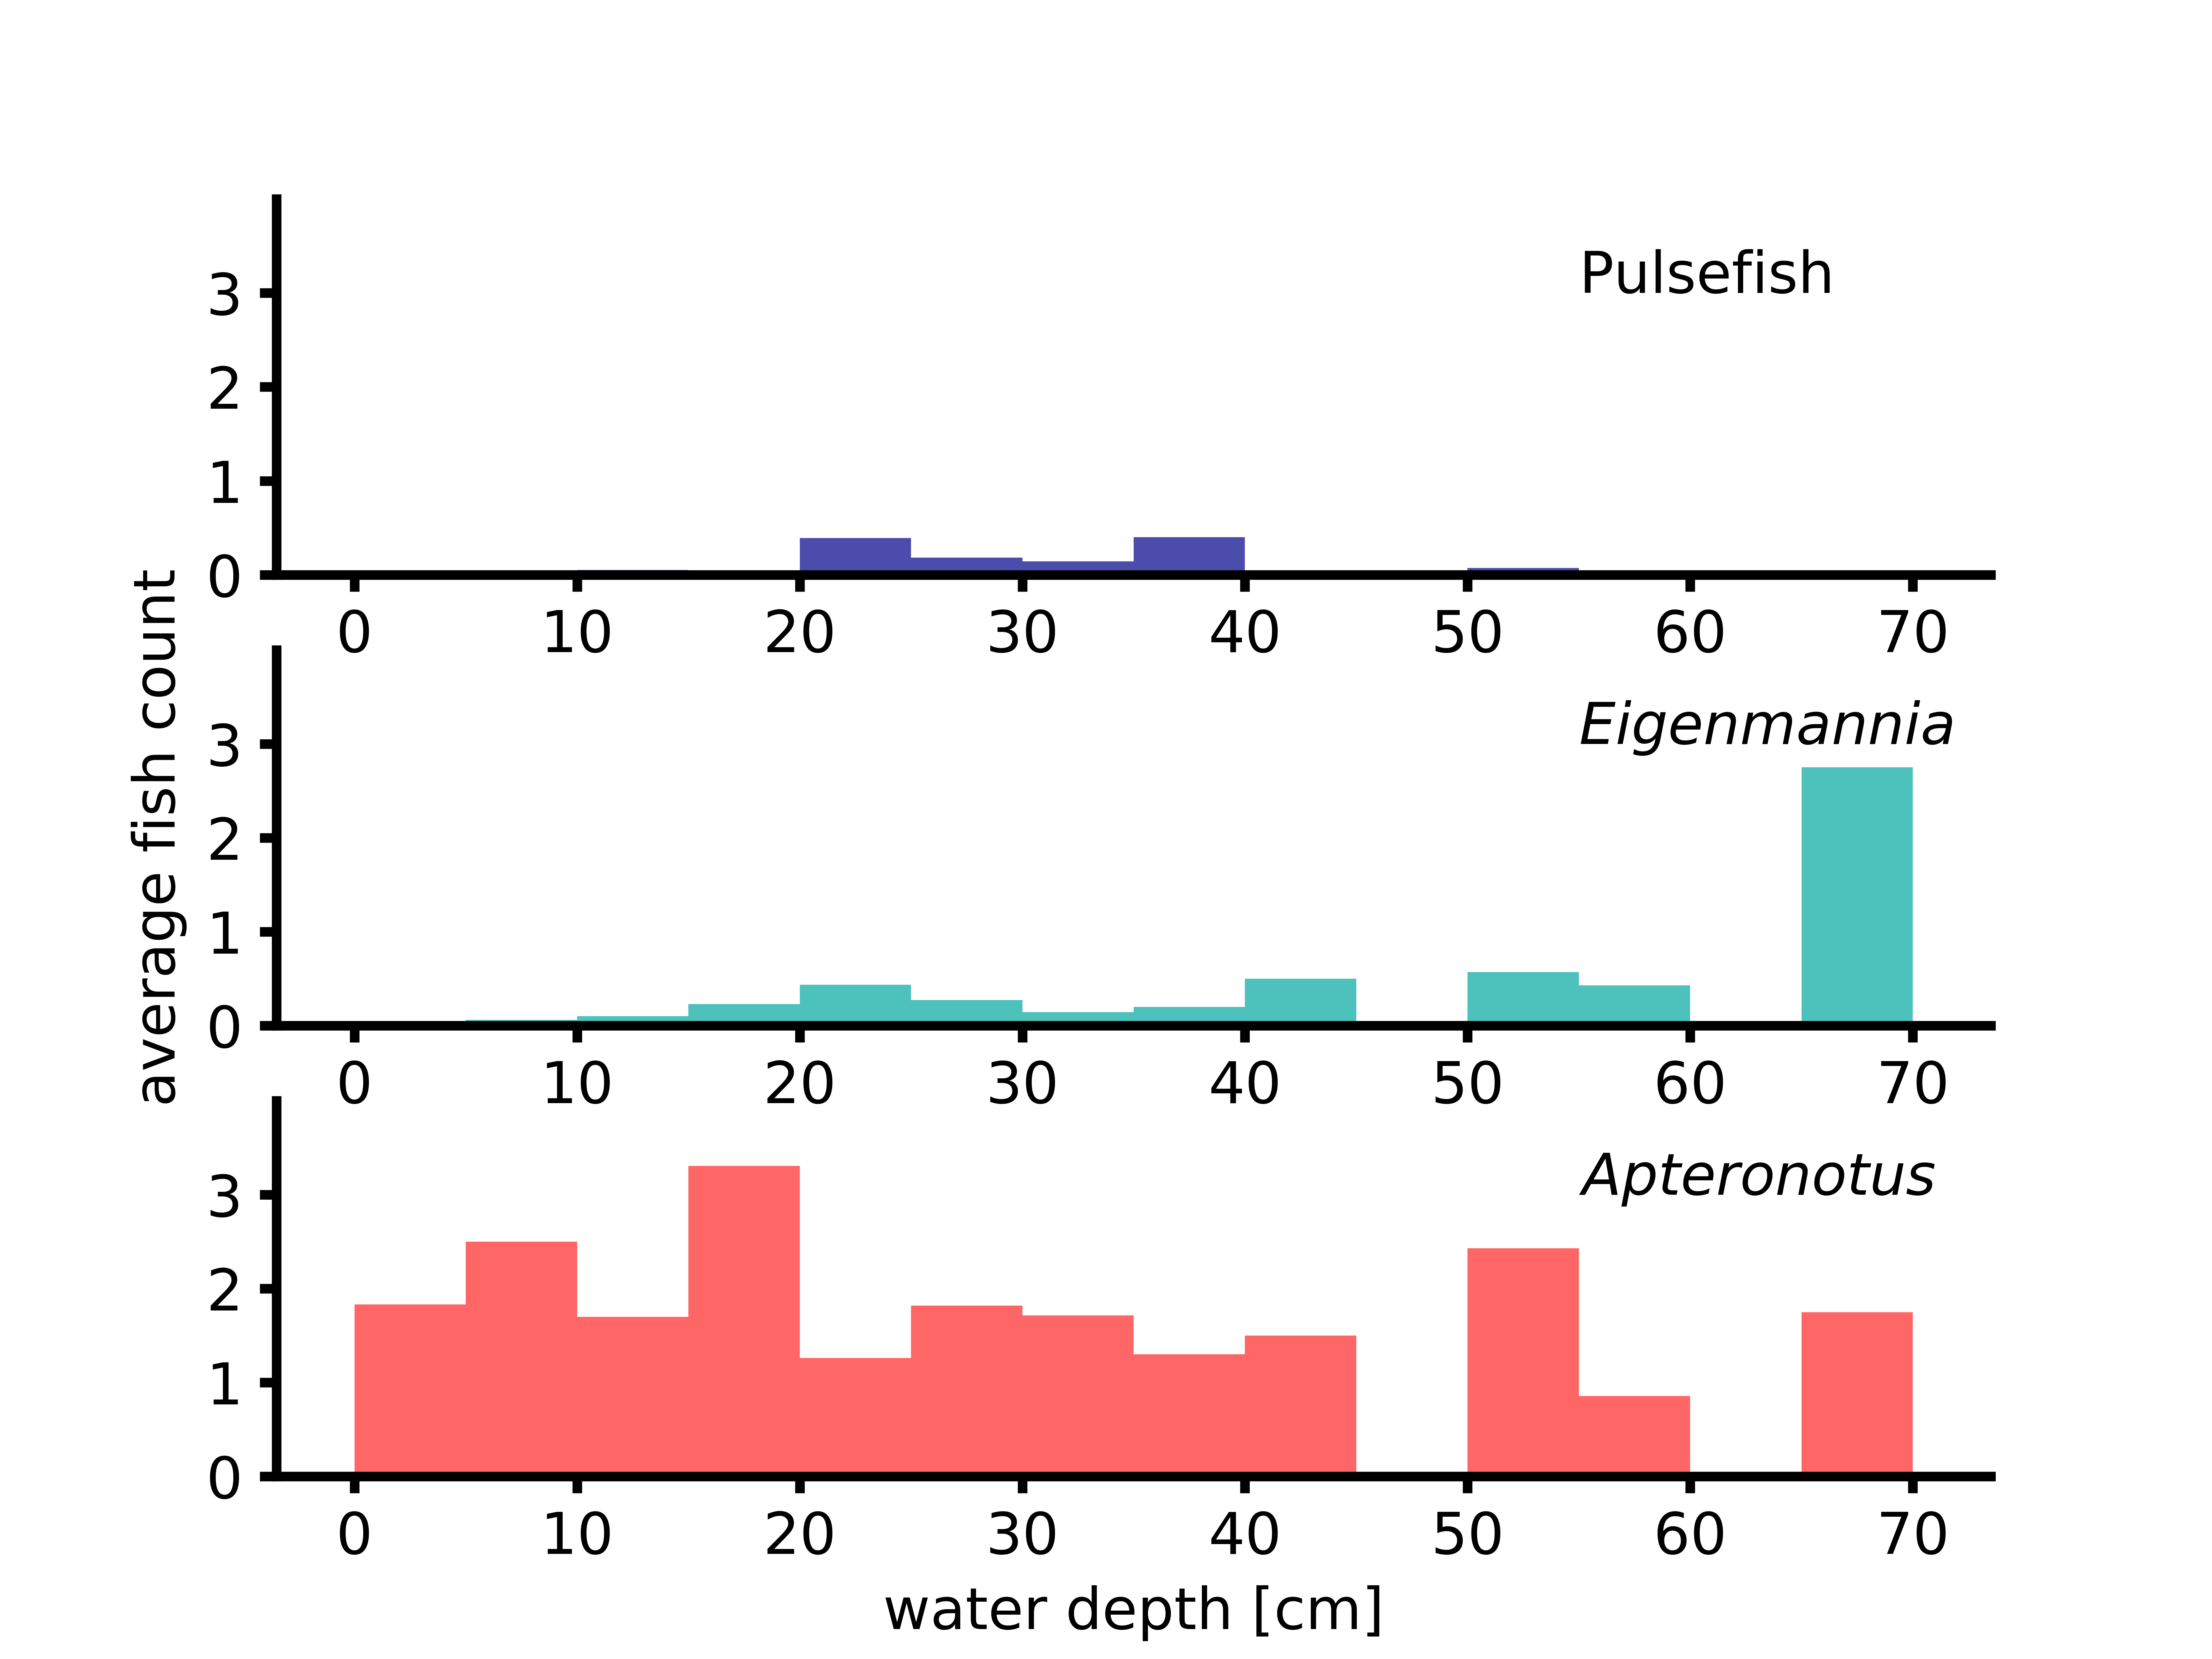
\includegraphics[width=0.9\textwidth]{pictures/Results/JULE_flow_depth2.png}
    \caption{\textbf{Occurrence of species dependent on water depth.} Shown is the average fish count for microhabitats within a certain range of water depth for pulsefish (blue), \textit{Apteronotus macrostomus} (red) and \textit{Eigenmannia virescens} (cyan). Water depths between 45~and 50~cm and 60~and 65~cm were not measured.}
    \label{fig:habitat_vs_depth}
\end{figure}

In addition to the occurrence of the different species or genera dependent on the water flow, their occurrence dependent on the water depth was investigated. Microhabitats with a water depth of 45~to 50~cm and 60~to 65~cm were not found. Regarding \textit{Apteronotus} and pulsefish, no preference for a certain water depth can be seen (fig.~\ref{fig:habitat_vs_depth}). Pulsefish were found in habitats with a water depth between 10~and 55~cm. \textit{Apteronoti} were found in microhabitats with a water depth ranging from a few centimeters up to 70~cm. Also \textit{Eigenmannia} was found within a large range of water depth (5~to 70~cm). In contrast to the other species or genera, \textit{Eigenmannia virescens} seemed to appear more frequently in habitats with a water depth between 65~and 70~cm.


% ----------------------------------------------
% Apteronoti (male / female) 
% ----------------------------------------------

\subsection{Dominance and habitat preferences in \textit{Apteronotus}}

\begin{figure}[H]
    \centering
    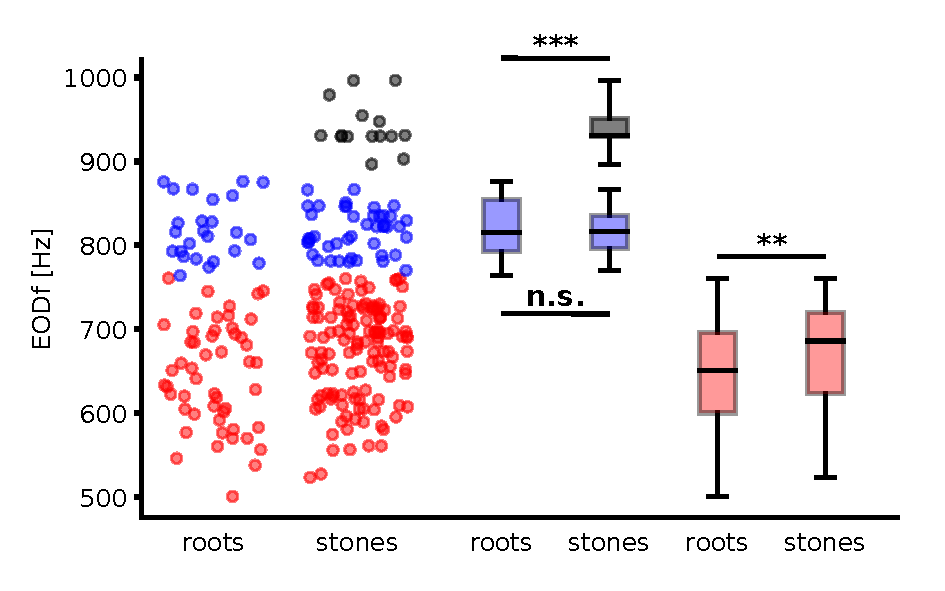
\includegraphics{pictures/Results/eod_habitat.pdf}
    \caption{\textbf{Distribution of the different EODfs of \textit{Apteronotus}, depending on the root and stone microhabitats.} Distribution of male and female \textit{A. macrostomus} in root- and stone-microhabitats. Based on the over-all EOD distribution in figure~\ref{fig:fish_count_eod}, males had an EODf above 762~Hz. The males were also divided into high frequency males and low frequency males at a threshold of 880~Hz.}
    \label{fig:habitat_vs_eod}
\end{figure}

It could be shown that many individuals of the species \textit{Apteronotus macrostomus} occurred in microhabitats made of stones or roots (fig.~\ref{fig:habitat_count_species}). This leads to the question how the different individuals occupy these different microhabitats and if there exists a relation between habitat selection and intra-specific dominance. Since intra-specific dominance is correlated with higher EOD frequencies, the individuals were grouped into three different categories dependent on the EODf: Females, males and high frequency males. According to the EOD frequency distribution in fig.~\ref{fig:fish_count_eod}B and the sexual dimorphism of the EODf, females were defined as having an EODf below 762~Hz. Consequently, recorded males had a EODf above 762~Hz and were further divided into low frequency and high frequency males (EODf~$>$~880~Hz).
Females and males were found in both, stone and root microhabitats (fig.~\ref{fig:habitat_vs_eod}). 
Females in stone and root microhabitats differed in their EOD frequency (Man-Whitney-U-Test: U~=~2385, p~=~0.004, Cohen's~d~=~-0.47). Compared with roots, in stony habitats were more females with higher EODf. The same trend can be seen looking at the males. For the low frequency males, no difference in EODf was found (Man-Whitney-U-Test: U~=~543.5, p~=~0.47). However, the high frequency and hence, the most dominant males, were exclusively found in stony microhabitats. 


\newpage
\section{Discussion}
% --------------------------------------------------
% all species, all habitats
% --------------------------------------------------

Our goal was to gain more information about the habitats and the ecology of different species of weakly electric fish. We characterised habitats and day shelter of different free living weakly electric fish in a network of river channels in the LLanos of the Orinoco basin, Meta, Colombia. Most of the examined habitats contained stones. Roots were also found frequently, whereas habitats containing mud or plants were less frequent (fig.~\ref{fig:habitat_count}). Within all examined habitats, weakly electric fish of three different species  or genera were found: wave-type fish of the species \textit{Apteronotus macrostomus} and \textit{Eigenmannia virescens} and pulse-type fish. The different species strongly differed in their frequency of occurrence (fig.~\ref{fig:habitat_count_species}). 
The three observed species preferred different microhabitats with different habitat characteristics, such as ground texture, water flow and water depth. Additionally, in \textit{A. macrostomus} a relation between dominance and habitat selection was found. 

\subsection{Habitat characteristics and preferences}

In general, different species show different preferences for habitats and shelter \citep{redsalmon1995,sherry1989redstarts,downes1998heat}. This also holds true for weakly electric fish \citep{Hopkins_74,HAGEDORN1985,lissmann1965activity}. Our results show different (micro-) habitat preferences of different species of weakly electric fish.
During the day, pulsefish preferred plants and roots as shelter, but were seldom found between stones (fig.~\ref{fig:habitat_vs_flow}). Since the preferred habitat characteristics of pulsefish occurred less frequent compared with other characteristics (fig.~\ref{fig:habitat_count}), the over-all count of these animals was quite low (fig.~\ref{fig:habitat_vs_eod}). \textit{Eigenmannia} showed a preference for mainly roots, which corresponds with the literature \citep{Hopkins_74}. Even though quite many microhabitats containing roots were found (fig.~\ref{fig:habitat_count}), the over-all count of individuals of this species was quite low compared with \textit{Apteronotus} (fig.~\ref{fig:habitat_vs_eod}). \textit{A. macrostomus} inhabited mostly stacked stones, but was also found in roots, rarely in plants. Stony habitats were by far the most frequent. Accordingly, \textit{Apteronotus} was by far the most frequent species. In pure sand habitats no fish were found. Since weakly electric fish are nocturnal animals \citep{lissmann1965activity} that seek shelter during the day \citep{Hopkins_74}, it seems likely that microhabitats containing solely sand are poor hiding places for the three occurring species.

Water flow and water depth can also play a role in shelter or habitat selection \citep{aadland1993stream}. Pulsefish inhibited habitats with either very low water flow or no water flow at all (fig.~\ref{fig:habitat_vs_flow}).  Most of them were found in water depth between 20~and 40~cm (fig.~\ref{fig:habitat_vs_depth}). However, a clear preference for a certain water depth can not be seen, due to a small amount of recorded pulse-fish in diverse microhabitats.
\textit{Apteronotus} also showed no preference, neither for water depth nor water flow. This species was found in a large flow range from stagnant to fast moving water and a variety of different water depths.
\textit{Eigenmannia} was mainly found in slow moving water, but some individuals were also found in high flow areas. Regarding the water depth, \textit{Eigenmannia virescens} is the only species that seemed to prefer deeper water. However, this effect might be caused by measurement inaccuracies. Sometimes, especially if several animals were found within a microhabitat, it was impossible to tell at which depth the individuals appeared. For each recording and microhabitat, the denoted water depth corresponds only with the position of one individual (chpt.~\ref{sec:recordings}).

Over-all, \textit{Apteronotus} seems to be more opportunistic, occurring in a variety of microhabitats regardless of water depth and flow. Other species of weakly electric fish were rarely found in the preferred habitat of \textit{Apteronotus} (stones). This could indicate that next to same sex conspecifics \citep{raab2019}, \textit{Apteronotus} may also defend its shelter against other species. This potential inter-specific dominance behavior of \textbf{Apteronotus} might have a strong influence on the habitat selection of the occurring  species. Another factor in influencing the habitat selection of the different species might be the occurrence of food sources. It is likely that different species prefer different aquatic insect larvae \citep{marrero1991notas}, which are likely to occur in different frequencies in the observed microhabitats. To better understand the habitat preferences of the different species,  it is necessary to know why certain shelter are selected. Investigating inter-specific dominance and natural foraging behavior of the different species, would be a good next step.

% --------------------------------------------------
% only apteronoti
% --------------------------------------------------

\subsection{Dominance and habitat preferences in \textit{Apteronotus}}

\begin{itemize}
    \item meisten Tiere Stones, dann Roots (sowohl männchen als auch weibchen)
    \item grund: steine bevorzugtes habitat - evtl guter shelter oder großes futteraufkommen oder weil wir einfach doppelt so viele Stein habitate hatten als root. Würde das argument eher auf die dominanz beziehen, weil es eine Aussage ist die die Daten bestätigen
    
    \item männchen: dominantereste tiere ausschließlich in steinen
    \item grund: sie setzen sich auf grund der dominanz gegen weniger dominante tiere durch
    \item daraus resultierende gründe: weil sie dominant sind haben sie bessere shelter oder mehr futter was dann deren überlebenschancen erhöht und somit die fitness, was sich wiederum auf die dominanz ausüben könnte...
    \item (body size ~ food intake, body size ~ dominance in Apteronotus leptorhynchus (K.D. Dunlap and L.M. Oliveri Retreat site selection and social organization in captive electric fish, Apteronotus leptorhynchus)
    \item innerhalb der weibchen: signifikanter unterschied zwischen EODf der individuen stein-vs-wurzel
    \item grund: vllt der selbe wie bei männchen weil dominanz 
    
    \item mögliche hinweise in diesen quellen dafür:
    \item Retreat site selection and social organization in captive electric fish, Apteronotus leptorhynchus, K.D. Dunlap and L.M. Oliveri, Journal of Comparative Physiology A, 188 (2002), pp. 469-477
    \item Electrocommunication signals in female brown ghost electric knife fish, Apteronotus leptorhynchus, S.K. Tallarovic and H.H. Zakon, Journal of Comparative Physiology A, 188 (2002), pp. 649-657
    \item \textcolor{red}{Allgemein: es scheint dominanz sowohl in männchen als auch weibchen zu geben, nur in männchen eben stärker ausgeprägt...}
    \item ZUKÜNFTIGE EXPERIMENTE:
    \item gründe warum steine ein besseres habitat sind als wurzel sollte genauer erforscht werden
    \item dominanz verhalten und habitat selection weiter untersuchen, auch zwischen weibchen 
    \item die Untersuchungsergebnisse von till im freiland sich anzu schauen 
\end{itemize}{}

% ergebnisse - zusammenfassung
\textit{Apterontus macrostomus} is mainly found in stacked stones followed by roots, which can be partially observed under laboratory conditions \citep{raab2019}. We found that high frequency males exclusively were found in stony habitats. Also the frequency of females in stony habitat was on average higher then the ones in root habitats. High EOD frequency is characteristic for dominance in male \textit{A. macrostomus}. The higher the frequency the more dominant the male with correlates with size of the fish \citep{triefenbach_zakon2003}. 

% conclusion
This suggests that stony habitats are preferred hiding place over the day. Stony habitats seem to be save shelters or offers high food availability and play a important role in the wild. This indicates that stacked stone 
Dominant males stay longer in their preferred day time habitat. But it is also observed that individuals switch to a new shelter in regular intervals mostly over night as well as over the day \citep{raab2019}. 


To better understand this, it is necessary to investigate the long term behavior in the wild over day and night to see which shelters are chosen.


 


%%%%%%%%%%%%%%%%%%%%%%%%%%%%%%%%%%%%%%%%%%%%%%%%%%%%%%%%%%%%%
%%%%%%%%%%%%%%%%%%%%%%%%%%%%%%%%%%%%%%%%%%%%%%%%%%%%%%%%%%%%%
\newpage
\addcontentsline{toc}{section}{References}
\bibliographystyle{abbrvnat}
\bibliography{references}

\newpage
\section{Supplementary}
% ___________________________________________________________

\textcolor{blue}{1. Abstract: Dominance between territorial males not only determines their fitness but might also influence selection of resting sites, because better resting sites might reduce physiological costs. The Gymnotiform weakly electric fish Apteronotus macrostomus is a nocturnal fish that evolved an electric organ derived from nerve cells as part of an active electrosensory system used for localization and communication. Electric organ discharges (EOD) generate species and individual specific EOD frequencies that are also indicating dominance among males. Dominant males with the highest EOD frequencies have been shown to defend the best shelters against subordinate males in staged laboratory settings. Here we correlate EOD frequencies and micro-habitat properties of A. macrostomus in its natural habitat, the Canocamoa river in the Meta region of the Llanos, Colombia, which drains into the Orinoco river. By using a fishfinder we recorded over 300 electric fish of various species in 139 different micro-habitats. Based on EOD waveforms and frequencies we identified A. macrostomus, which was the most abundant species. During the day, we found A. macrostomus in various habitats with distinct water velocities ranging from 0 to 2.5 m/s. The fish preferred stacked stones and root formations for shelter. Males with the highest EOD frequencies were exclusively found in stacked stone habitats, indicating that these are the best shelters and are successfully defended by the most dominant males. Thus, we found that effects of dominance on shelter selection as shown previously in the lab also play a role under natural conditions.}\\

\textcolor{blue}{2. abstract: There are arguably few places in the world that can claim a biodiversity as high as Colombia’s. Colombia’s unique ecosystem is comprised of innumerous animal species that have adapted to a diverse set of habitats. Among these, weakly electric fish make up 70\% of the biomass of the respective native fish fauna. The south American weakly electric fish of the order Gymnotiformes evolved an electric organ which cells discharge simultaneously and create an electric field around the animal. They use this electric organ discharge (EOD) for electrolocation and communication. While this electrosensory system is well researched in the lab, much less is known about the ecology and ethology of these fishes. We assessed habitat conditions and habitat preferences of Gymnotiform fishes in the Rio Canocamao of the Orinoco basin, in the Reserva el Caduceo in San Martin, Meta, Colombia. Across this tropical grassland plane stretches a widely ramified network of river channels with pastures and secondary tropical forests in between. The self generated electric fields were used to record and detect individual electric fish in their natural environment. We categorized their distribution across a wide range of natural river habitats that we characterized by water flow, water depth and structure of the river bed. Within 139 recordings we detected more than 300 weakly electric fish of various species. Based on EOD properties and frequencies extracted from the recordings, we classified the fish into four species groups: wave-type fish of the genera Apteronotus, Eigenmannia, and Sternopygus and pulse-type fish. These species strongly differed in their abundance and habitat preference. By far, Apteronotus was the most frequent and clearly preferred to hide between stacked stones during the day. Eigenmannia tended to stay inside root formations. Pulse-type fish preferred to hide in water plants. Eigenmannia and pulse-fish were found in habitats with low water speeds (lesser than   0.5 m/s), whereas Apteronotus was also found in much faster flowing waters. The diversity of occupied niches suggests strong physiological and behavioral adaptations of the different species of weakly electric fish.}

\end{document}
